\documentclass{beamer}
\usepackage[lithuanian]{babel}
\usepackage[utf8x]{inputenc}
\usepackage[L7x]{fontenc}
\usepackage{lmodern}
\usepackage{caption}
\usepackage{subfig}
\usepackage{graphicx}
\usepackage{tikz}
\usetikzlibrary{arrows}

\let\oldshorttitle\insertshorttitle
\renewcommand*\insertshorttitle{
    \leftskip=0.4cm
\oldshorttitle\hfill \insertframenumber\,/\,\inserttotalframenumber
}

\usetheme{Dresden}

\title[Žinių išgavimas]{Automatizuotas žinių išgavimas, sistemos}
\author[M. Norkin]{Maksim Norkin, AKSfm-15}
\institute[VGTU Elektronikos fakultetas]{
    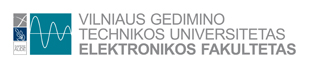
\includegraphics[height=30px]{img/logo.jpg}\\
    Vilniaus Gedimino technikos universitetas\\
    Elektronikos fakultetas\\
    Elektroninių sistemų katedra\\
    \texttt{maksim.norkin@stud.vgtu.lt}
}

\begin{document}

    \begin{frame}
        \titlepage
    \end{frame}

    \begin{frame}{Istorija}

        \begin{itemize}
            \item $\sim$ 1960m. Primityvios bylos
            \item $\sim$ 1970m. Reliacinės, hierarchinės sistemos
            \item $\sim$ 1980m. Duomenų analizės sistemos
            \item $\sim$ 1990m. Internetinės duomenų bazės
            \item $\sim$ 2000m. Daug duomenų
        \end{itemize}

    \end{frame}

    \begin{frame}[allowframebreaks]{Žinios}

        Žinių atradimo procesas:

        \begin{itemize}
            \item Valymas
            \item Integravimas
            \item Pasirinkimas
            \item Transformavimas
            \item Išgavimas
            \item Įvertinimas
            \item Pateikimas
        \end{itemize}

        \framebreak

        Išgaunamos žinios:

        \begin{itemize}
            \item Duomenų bazės
            \item Duomenų saugyklos
            \item Transakcijos duomenis
            \item Kiti duomenys
        \end{itemize}

    \end{frame}

    \begin{frame}{Modeliai}

        \begin{itemize}
            \item Charakterizavimas ir diskriminavimas
            \item Dažniniai modeliai ir koreliacijos
            \item Klasifikavimas ir regresija
            \item Grupinė analizė
            \item Išskirčių analizė
        \end{itemize}

    \end{frame}

    \begin{frame}{Technologijos}

        Naudojamos technologijos

        \begin{itemize}
            \item Statistika
                \begin{itemize}
                    \item Pagrindas analizei
                \end{itemize}
            \item Mašininis mokymas
                \begin{itemize}
                    \item Prižiūrimas
                    \item Neprižiūrimas
                    \item Dalinai prižiūrimas
                    \item Aktyvus
                \end{itemize}
            \item Duomenų bazės sistemos ir duomenų saugyklos
                \begin{itemize}
                    \item Išplėtimo galimybė
                    \item Semantinė duomenų analizė
                \end{itemize}
        \end{itemize}

    \end{frame}

    \begin{frame}{Pritaikymai}

        \begin{itemize}
            \item Naudotojų poreikių analizė
                \begin{itemize}
                    \item Geresnis suvokimas apie klientus
                    \item Apie rinką
                    \item Poreikį
                \end{itemize}
            \item Akcijų biržos kainų spėjimas
                \begin{itemize}
                    \item Greitas pirkimas / pardavimas
                \end{itemize}
            \item Paieškos varikliai
        \end{itemize}

    \end{frame}

    \begin{frame}{Išvados}

        \begin{itemize}
            \item Išgauti įdomius modelius iš didelio duomenų kiekio
            \item Daugelio dimensijų požiūris į duomenis
            \item Labai daug sėkmingų įgyvendinimų
        \end{itemize}

    \end{frame}

\end{document}